\section{Data Generation and Training}
\label{sec:training}

Training a reusable scorer requires examples that separate process behavior from the way a net happens to represent it. It also requires trustworthy targets: synthetic corruption tells us how an observation was produced, but not necessarily its cheapest explanation. This section describes the complete path from a generated behavior family to input tensors, exact alignment targets, and parameter updates. All generation and loss details needed to understand the reference model are integrated here.

\subsection{Why Generate Behavior Families?}
\label{sec:families}

An isolated pair of a random net and a noisy trace would teach the network about one representation at a time. It would give much less control over whether a performance change comes from different behavior or merely different routing. A \emph{behavior family} addresses this by grouping two nets with the same complete visible language and two shared observations:
\begin{equation}
 \mathcal B=(SN_1,SN_2,\sigma_1,\sigma_2),\qquad
 \mathcal L(SN_1)=\mathcal L(SN_2).
 \label{eq:family}
\end{equation}
Each family expands into four supervised inputs, $(SN_r,\sigma_k)$ for $r,k\in\{1,2\}$. Both representations see exactly the same observations. Figure~\ref{fig:family} shows this expansion and the checks that precede writing the rows.

The entire family belongs to one split before expansion. This avoids placing two views of the same generated family in training and test. It does not make all visible languages, motifs, or net topologies disjoint across splits: independently generated families can repeat the controlled structures. The test split measures new family instances within this generator, not transfer to wholly unseen motif classes.

\begin{figure}[tb]
\centering
\begin{tikzpicture}[x=1cm,y=1cm]
\node[box,text width=30mm] (plan) at (1.6,0) {assign split\\choose motif};
\node[box,text width=30mm] (nets) at (5.3,0) {build two Petri nets\\$SN_1$ and $SN_2$};
\node[verifybox,text width=30mm] (check) at (9,0) {check languages\\and structure};
\draw[flow] (plan) -- (nets); \draw[flow] (nets) -- (check);
\node[box,text width=30mm] (pool) at (9,-1.9) {select two traces\\from clean pool};
\node[warnbox,text width=30mm] (noise) at (5.3,-1.9) {apply edits once\\share $\sigma_1,\sigma_2$};
\node[box,text width=30mm] (rows) at (1.6,-1.9) {form four inputs\\$(SN_r,\sigma_k)$};
\draw[flow] (check) -- (pool); \draw[flow] (pool) -- (noise); \draw[flow] (noise) -- (rows);
\node[verifybox,text width=30mm] (teacher) at (1.6,-3.9) {exact alignments\\one per input};
\node[verifybox,text width=30mm] (replay) at (5.3,-3.9) {replay witnesses\\check equal costs};
\node[learnbox,text width=30mm] (save) at (9,-3.9) {accept whole family\\store inputs + targets};
\draw[flow] (rows) -- (teacher); \draw[flow] (teacher) -- (replay); \draw[flow] (replay) -- (save);
\node[annotation,anchor=west,text width=105mm] at (0,-5.3) {If a required check fails, replace the attempted family with another of the same planned motif. Corruption history never becomes a neural input.};
\end{tikzpicture}

\caption{Data generation as a sequence of explicit checks. One family supplies two behaviorally equivalent representations and two observations shared across them. Each of the four rows receives its own exact witness. A family is written only after all rows pass, keeping both the split assignment and the planned motif balance intact.}
\label{fig:family}
\end{figure}

Before generating nets, a deterministic quota assigns the requested number of families to four equally weighted motifs. Minimum family counts are reserved per motif, remaining slots are distributed by the weights, and the plan is shuffled with a split-specific seed. If a generation attempt fails, another family index is tried for the same planned motif. This prevents rejection from silently shifting the corpus toward easier model classes. The global reference seed is 13; separate seeds derived from the split and family index control structure, representation, and corruption.

\subsection{Four Motifs and Their Representation Pairs}
\label{sec:motifs}

The motifs target distinct reasons why a label sequence may be difficult to align. Table~\ref{tab:motifs} specifies their visible core languages. The three controlled motifs append two fresh activities shared by both representations. If their labels are $u,v$, the complete language is $\{wuv:w\in\mathcal L_{\mathrm{core}}\}$. Fresh labels prevent the suffix from introducing another core ambiguity. The implementation selects the first unused activity names: the duplicate/silent and M motifs append $D,E$, while the concurrency motif appends $C,D$.

\begin{table}[tb]
\caption{Motif design. The listed languages omit the shared suffix for the three controlled motifs. ``Canonical'' identifies the generator's fixed block compiler.}
\label{tab:motifs}
\centering
\begin{tabularx}{\linewidth}{@{}lY Y@{}}
\toprule
Motif & Core behavior & Representation pair\\
\midrule
Ordinary tree & Sampled tree language & Canonical block net and isomorphic identifier renaming.\\
Duplicate/silent & $AB$, $AC$ & Two $A$ transitions that select a branch; one $A$ followed by invisible routing.\\
Concurrency & $AB$, $BA$ & True parallel execution; explicit choice between the two sequences.\\
M pattern & $B$, $AC$, $CA$ & XOR of $B$ and parallel $A,C$; non-free-choice M net.\\
\bottomrule
\end{tabularx}
\end{table}

\subsubsection{Ordinary Trees and Identifier Renaming}

This pair tests whether a candidate depends on incidental naming. A random process tree has 4--12 visible leaf occurrences and depth at most six. Sequence, XOR, and AND have selection probabilities $0.4$, $0.3$, and $0.3$. The alphabet size is approximately 70\% of the visible leaf count, so different leaves can carry the same label. The compiler maps leaves to visible transitions, sequences to linked fragments, XOR branches to shared entry and exit places, and AND to invisible split/join routing.

The second net is an isomorphic copy with renamed place and transition identifiers. Labels, arcs, markings, and weights remain unchanged under the corresponding bijections. Its firing possibilities and optimal costs are therefore unchanged. Sorting the new identifiers can, however, change an unguided tie-break. This pair distinguishes an improvement in handling identifiers from an improvement on a new process behavior.

\subsubsection{Duplicate Prefix and Silent Routing}

This pair isolates a choice that may have to be made before its distinguishing event arrives. In the duplicate-prefix net, two enabled transitions are both labeled $A$. One leads to $B$ and the other to $C$. Firing $A$ therefore commits to a branch. In the silent-routing net, there is one shared $A$ transition followed by two invisible alternatives that enable $B$ or $C$. Both nets generate $AB$ or $AC$ before the common suffix, but the visible ambiguity occurs at a different point. Figure~\ref{fig:duplicatepair} draws both cores.

For an observation beginning with $A,C$, selecting the appropriate duplicate $A$ requires looking beyond the current event. The silent-routing representation can postpone its branch selection until trying to enable $C$. If guidance helps mainly on the first net, that is evidence about early ambiguity, rather than a universal advantage over the same decoder.

\begin{figure}[tb]
\centering
\begin{tikzpicture}[x=1cm,y=1cm]
\node[paneltitle] at (0,1.8) {A. Duplicate prefix: choose the branch while firing $A$};
\node[place] (a0) at (.35,0) {};\fill[ink] (a0) circle (.065);
\node[transition] (al) at (1.85,.7) {$A$};
\node[transition] (ar) at (1.85,-.7) {$A$};
\node[place] (pl) at (3.25,.7) {};
\node[place] (pr) at (3.25,-.7) {};
\node[transition] (b) at (4.65,.7) {$B$};
\node[transition] (c) at (4.65,-.7) {$C$};
\node[place] (f) at (6.1,0) {};
\foreach \a/\b in {a0/al,a0/ar,al/pl,ar/pr,pl/b,pr/c,b/f,c/f}\draw[arc] (\a) -- (\b);
\node[annotation,above=2mm of al] {$A_L$};\node[annotation,below=2mm of ar] {$A_R$};
\node[box,text width=28mm] (suffix) at (8.25,0) {shared suffix\\$D$ then $E$};
\draw[flow] (f) -- (suffix);
\node[place,double] (end) at (10.35,0) {};\draw[flow] (suffix) -- (end);
\node[paneltitle] at (0,-2) {B. Silent routing: postpone the choice until after $A$};
\node[place] (b0) at (.35,-3.5) {};\fill[ink] (b0) circle (.065);
\node[transition] (a) at (1.45,-3.5) {$A$};
\node[place] (mid) at (2.55,-3.5) {};
\node[silent] (tl) at (3.7,-2.8) {$\tau$};
\node[silent] (tr) at (3.7,-4.2) {$\tau$};
\node[place] (bl) at (4.85,-2.8) {};
\node[place] (br) at (4.85,-4.2) {};
\node[transition] (bb) at (6,-2.8) {$B$};
\node[transition] (bc) at (6,-4.2) {$C$};
\node[place] (bf) at (7.15,-3.5) {};
\foreach \a/\b in {b0/a,a/mid,mid/tl,mid/tr,tl/bl,tr/br,bl/bb,br/bc,bb/bf,bc/bf}\draw[arc] (\a) -- (\b);
\node[box,text width=17mm] (s2) at (8.75,-3.5) {$D$ then $E$};
\node[place,double] (e2) at (10.35,-3.5) {};
\draw[flow] (bf) -- (s2);\draw[flow] (s2) -- (e2);
\end{tikzpicture}

\caption{Equal visible languages with different decision points. Top: choosing a concrete $A$ transition commits to $B$ or $C$. Bottom: a shared $A$ precedes invisible branch routing. The appended suffix $D,E$ is identical in both nets. The visible language is $\{ABDE,ACDE\}$, although transition identities and silent moves differ.}
\label{fig:duplicatepair}
\end{figure}

\subsubsection{Parallelism and Explicit Interleaving}

This pair tests a change in the representation of concurrency. One net uses an invisible split to enable $A$ and $B$ in parallel, followed by a join. The other uses an XOR between the sequences $AB$ and $BA$. Their complete visible traces coincide, but their causal structures differ: simultaneous availability in one representation becomes a choice between sequential executions in the other. The equivalence is therefore trace-language equivalence, not equivalence of partial-order behavior. This distinction matters when interpreting representation agreement as evidence of transfer.

\subsubsection{Block Structure and the Non-Free-Choice M Pattern}

This pair tests a conflict between transitions with different input places. The block representation is $\operatorname{XOR}(B,\operatorname{AND}(A,C))$. In the M representation, an invisible split places one token in each of two places. $A$ consumes the first, $C$ consumes the second, and $B$ consumes both. Therefore $B$ conflicts with both $A$ and $C$, while $A$ and $C$ can occur in either order. The presets of conflicting transitions are unequal, giving the non-free-choice structure. Appropriate output places and a join complete the $A,C$ branch. Figure~\ref{fig:structuralpairs} shows the token-level construction together with the parallelism pair.

\begin{figure}[tb]
\centering
\begin{tikzpicture}[x=1cm,y=1cm]
\node[paneltitle] at (0,1.5) {A. Parallel execution and explicit interleavings};
\node[place] (s) at (.25,0) {};\fill[ink] (s) circle (.06);
\node[silent] (split) at (1.15,0) {$\tau$};
\node[place] (p) at (2.2,.65) {};
\node[place] (q) at (2.2,-.65) {};
\node[transition] (a) at (3.25,.65) {$A$};
\node[transition] (b) at (3.25,-.65) {$B$};
\node[place] (pa) at (4.3,.65) {};
\node[place] (pb) at (4.3,-.65) {};
\node[silent] (join) at (5.35,0) {$\tau$};
\node[place,double] (f) at (6.25,0) {};
\foreach \a/\b in {s/split,split/p,split/q,p/a,q/b,a/pa,b/pb,pa/join,pb/join,join/f}\draw[arc] (\a) -- (\b);
\node[box,text width=30mm] at (8.65,0) {equivalent visible choice\\$\operatorname{XOR}(AB,BA)$};
\node[annotation] at (3.25,-1.4) {split produces two tokens; join requires both};
\node[paneltitle] at (0,-2.2) {B. The M pattern and its block representation};
\node[place] (s2) at (.25,-4) {};\fill[ink] (s2) circle (.06);
\node[silent] (sp) at (1.15,-4) {$\tau$};
\node[place] (p2) at (2.2,-3.2) {};
\node[place] (q2) at (2.2,-4.8) {};
\node[transition] (a2) at (3.6,-2.85) {$A$};
\node[transition] (b2) at (3.6,-4) {$B$};
\node[transition] (c2) at (3.6,-5.15) {$C$};
\node[place] (pa2) at (4.9,-2.85) {};
\node[place] (pc2) at (4.9,-5.15) {};
\node[silent] (j2) at (6,-4) {$\tau$};
\node[place,double] (f2) at (7,-4) {};
\foreach \a/\b in {s2/sp,sp/p2,sp/q2,p2/a2,q2/c2,p2/b2,q2/b2,a2/pa2,c2/pc2,pa2/j2,pc2/j2,j2/f2}\draw[arc] (\a) -- (\b);
\draw[arc,preaction={draw=white,line width=3pt}] (b2.east) -- (4.15,-4) -- (4.15,-5.8) -- (7,-5.8) -- (f2.south);
\node[box,text width=24mm] at (9.15,-4) {equivalent block\\$\operatorname{XOR}(B,$\\$\operatorname{AND}(A,C))$};
\node[annotation,anchor=west] at (0,-6.35) {$B$ needs both tokens; firing $A$ or $C$ prevents $B$ from firing.};
\end{tikzpicture}

\caption{Two additional changes of representation. The parallel core and the explicit interleaving expression both admit $AB$ and $BA$. In the M core, $B$ consumes both central tokens, while $A$ and $C$ consume one each and later join; its visible language is $\{B,AC,CA\}$. The right-hand expressions denote the corresponding block structures. Shared fresh suffixes are omitted.}
\label{fig:structuralpairs}
\end{figure}

\subsection{Checking Behavioral Equivalence and Usable Structure}
\label{sec:equivalence}

The representation checks protect the interpretation of a family. If the two nets admitted different visible traces, a cost difference could be semantically correct rather than a representation effect. The generator enumerates complete visible traces and records whether enumeration finishes. Default limits are 5000 explored states, 10,000 complete traces, and visible length 20, with an additional firing bound to prevent unbounded invisible exploration. A comparison is labeled \emph{exact} only if neither enumeration is truncated. A matching bounded prefix is not treated as proof of full language equality.

Generation rejects mismatching languages, an empty complete language, an unreachable final marking, or a dead transition. Here dead means that the structural exploration finds no reachable firing of that transition. These checks are useful filters, but should not be read as a general proof of every workflow-net soundness property for arbitrary inputs. The default training configuration also rejects families whose equivalence check is only bounded. All accepted rows in the reference training, validation, and test corpus have exact language certificates within the configured bounds.

The cost comparison used later has a formal rationale. Let $d_{\mathrm{ID}}(\sigma,w)$ be insertion/deletion distance, with unit cost for each inserted or deleted visible activity. With the costs in Table~\ref{tab:moves},
\begin{equation}
 \delta(\sigma,SN)=\min_{w\in\mathcal L(SN)}d_{\mathrm{ID}}(\sigma,w).
 \label{eq:languagecost}
\end{equation}
Every legal alignment selects a complete visible model word and a corresponding sequence of insertions, deletions, and matches. Conversely, such an edit sequence can be combined with a firing sequence for that word, inserting its zero-cost invisible moves. Thus language-equivalent nets have equal optimal visible-deviation costs, even though their optimal transition sequences may differ. This equality would require re-examination if costs depended on transition identity or charged invisible routing.

\subsection{Producing Observations by Trace Corruption}
\label{sec:corruption}

Corruption creates deviations without changing the reference process. For each accepted family, the enumerated language is sorted. If it contains more than 16 words, the family random generator selects 16 indices and restores them to language order. Otherwise the whole language is retained. The first two entries of this pool supply clean traces, wrapping around when only one entry is available. These choices and their corruption are deterministic given the configured seeds.

Each observation is kept clean with probability $0.2$. Otherwise it receives one, two, or three edits with probabilities $0.5$, $0.3$, and $0.2$. Table~\ref{tab:noise} lists the operation weights. Operations are drawn again after each edit and act on the current trace. Inapplicable operations, such as a swap on a one-event trace, fall back to insertion of the outside label \texttt{\_\_OOD\_\_}. Traces are capped at length 128. The realized frequencies can therefore differ from the nominal weights, especially for short observations.

\begin{table}[tb]
\caption{Trace-corruption operations. Examples start from $ABDE$ and illustrate individual edits; multi-edit traces apply several operations in sequence. Weights are conditional on drawing an edit operation.}
\label{tab:noise}
\centering
\begin{tabularx}{\linewidth}{@{}l c Y l@{}}
\toprule
Operation & Weight & Effect & Example\\
\midrule
Delete & .15 & Remove an event. & $ADE$\\
Insert & .15 & Insert a label from the family alphabet. & $ABBDE$\\
Substitute & .15 & Replace an event label. & $ACDE$\\
Swap & .15 & Exchange neighboring events. & $BADE$\\
Repeat & .15 & Duplicate one event. & $ABDEE$\\
Prefix truncation & .10 & Remove a beginning segment. & $DE$\\
Suffix truncation & .10 & Remove an ending segment. & $AB$\\
Outside insertion & .05 & Insert the special outside label $X$. & $ABXDE$\\
\bottomrule
\end{tabularx}
\end{table}

The same corrupted observation is then paired with both nets. This is essential to the comparison: applying different noise to the two representations would confound behavior with observation quality. The corruption history is metadata, not a neural input and not the alignment target. An edit can produce another fitting trace; several edits can cancel or admit an explanation cheaper than undoing them. For example, substituting $C$ for $B$ in $ABDE$ produces $ACDE$, which still fits the duplicate/silent family. Exact alignment is therefore performed after corruption.

\subsection{Exact Supervision and Family-Level Acceptance}
\label{sec:teacher}

Each expanded row is sent to the PM4Py state-equation A* teacher with transition-aware output. The reference generation imposes no per-trace timeout. Results are cached within a split using a signature of the net, the observed sequence, and the cost-model version. Caching reduces repeated teacher work without changing the targets. A different representation still requires its own concrete transition witness.

Every exact witness is replayed independently. The initializer requires an optimal result, checks all moves and both projections, and verifies that the paired nets give equal optimal costs for the same observation when their language equivalence was exact. Rows are buffered until the entire family passes; a failure replaces the family rather than writing only its successful rows. For the reference corpus, the manifest records 25 generation-time \texttt{ValueError} attempts that were replaced. It records no exact-alignment, replay, or paired-cost rejection. These are observations about this run, not a guarantee that future configurations cannot fail those gates.

From one optimal witness $\gamma^*$, the code derives three move targets. The synchronous target $y_i$ is the zero-based index of the transition used for event $i$, or $-1$ when there is no active synchronous target. The binary target $q_i$ is one exactly when the event is a log move. The binary target $b_j$ is one when transition $t_j$ occurs at least once as a model move anywhere in $\gamma^*$. Invisible model moves are included in $b$. This last target does not record the position or multiplicity of model moves, matching the deliberately coarse vector $M$.

Teacher identity is not unique when several alignments are optimal. The generator uses one particular witness. For the duplicate-prefix motif, it further masks all synchronous targets when the observation contains both distinguishing labels $B,C$ or neither. This is the implemented heuristic for avoiding ambiguous identity supervision, not a general theorem characterizing all unique optima. Log, model, and cost targets remain active, and the witness itself remains in the stored row.

\subsection{A Complete Worked Training Row}
\label{sec:trainingrow}

A concrete row helps separate input information from the answer supplied during training. Consider stored sample \texttt{train-000048}. Starting from $ABDE$, the generator swaps the final events and substitutes $C$ for $B$, yielding $\sigma=\langle A,C,E,D\rangle$. Its duplicate-prefix net is the upper representation of Figure~\ref{fig:duplicatepair}, followed by the suffix. Write $A_L,A_R$ for its two $A$ transitions, with $A_L$ leading to $B$ and $A_R$ to $C$.

The place order is $(p_D,p_E,p_0,p_f,p_L,p_R)$ and the transition order is $(D,E,A_L,A_R,B,C)$. The core ends at $p_f$, followed by $D$ to $p_D$ and $E$ to $p_E$; the final marking is $[p_E]$. In these orders, the numerical feature matrices are
\begin{equation}
 X_P=\begin{bmatrix}
 0&0&1&1&2\\0&1&1&0&1\\1&0&0&2&2\\
 0&0&2&1&3\\0&0&1&1&2\\0&0&1&1&2
 \end{bmatrix},\qquad
 X_T=\begin{bmatrix}
 0&1&1&1&0&0\\0&1&1&1&0&0\\0&1&1&1&0&0\\
 0&1&1&1&0&0\\0&1&1&1&0&0\\0&1&1&1&0&0
 \end{bmatrix}.
 \label{eq:concretefeatures}
\end{equation}
Every transition has the same local feature row, yet the graph connections and labels differ. This demonstrates why local degrees alone cannot resolve the duplicate choice.

The graph uses place indices $0,\ldots,5$ and transition-node indices $6,\ldots,11$. Table~\ref{tab:concreteedges} specifies all edges compactly. For each triple $(p,t,q)$, insert edges $(p,t),(t,p),(t,q),(q,t)$ with types $(0,2,1,3)$. Thus $E$ has 24 columns and $r$ repeats this four-type sequence six times. This explicitly recovers the arc information that distinguishes the otherwise equal rows of $X_T$.

\begin{table}[tb]
\caption{Full edge specification for the worked input. The readable transition name identifies a row; the three integers are graph-node indices in Equation~\eqref{eq:concretefeatures}.}
\label{tab:concreteedges}
\centering
\begin{tabular}{@{}lrrr@{}}
\toprule
Transition & Input place $p$ & Transition node $t$ & Output place $q$\\
\midrule
$D$ & 3 & 6 & 0\\
$E$ & 0 & 7 & 1\\
$A_L$ & 2 & 8 & 4\\
$A_R$ & 2 & 9 & 5\\
$B$ & 4 & 10 & 3\\
$C$ & 5 & 11 & 3\\
\bottomrule
\end{tabular}
\end{table}

The label IDs and exact compatibility matrix are
\begin{align}
 z_T&=(2587,4475,8075,8075,6408,5878),\nonumber\\
 z_\sigma&=(8075,5878,4475,2587),\label{eq:concreteids}\\
 C&=\begin{bmatrix}
 0&0&1&1&0&0\\0&0&0&0&0&1\\0&1&0&0&0&0\\1&0&0&0&0&0
 \end{bmatrix}.\label{eq:concretemask}
\end{align}
The first event can match either $A$ transition. The third event is compatible with $E$, even though $E$ is not enabled initially. The separate position indices $(0,1,2,3)$ are added by the trace encoder. Equations~\eqref{eq:concretefeatures}--\eqref{eq:concretemask} and Table~\ref{tab:concreteedges} specify every component of $X$; no clean trace or exact cost is among these inputs.

The stored teacher witness is
\begin{equation}
 \gamma^*=\langle(A,A_R),(C,C),(E,\skipmove),(D,D),(\skipmove,E)\rangle,
 \qquad\delta=2.
 \label{eq:concretewitness}
\end{equation}
It takes the branch consistent with $C$, skips the early $E$, synchronizes $D$, and finishes with a model move $E$. Another optimum could insert $D$ before synchronizing $E$ and then skip the final observed $D$. The chosen witness gives
\begin{equation}
 y=(3,5,-1,0),\qquad q=(0,0,1,0),\qquad b=(0,1,0,0,0,0).
 \label{eq:concretetargets}
\end{equation}
These arrays and $\delta$ are the supervision. In particular, target $y_1=3$ names $A_R$ in the stored zero-based transition order; it is not activity ID 3. This distinction is important when implementing transition-aware learning.

\subsection{Training-Time Relabeling and Corpus Composition}

Label relabeling discourages the scorer from solving controlled examples by memorizing a small set of synthetic IDs. On every training visit, probability $0.5$ triggers a consistent random remapping of distinct nonzero IDs in the net and trace to distinct values in $\{1,\ldots,8191\}$. The graph, exact compatibility mask, and targets remain unchanged. For example, mapping the IDs for $A,B,C,D,E$ to $101,205,309,413,517$ would give $z_T'=(413,517,101,101,205,309)$ and $z_\sigma'=(101,309,517,413)$. This example illustrates an augmentation, not a recorded random draw.

ID zero stays reserved for invisible transitions, and existing hash collisions remain collisions. Because embeddings differ across IDs, this augmentation encourages robustness but does not prove invariance under every label renaming. Validation and test use their original hashed IDs, and dropout is disabled there. The reference split sizes appear in Table~\ref{tab:splits}. The test traces average 3.6 events and their exact costs range from zero to seven, so this is a small controlled corpus rather than a comprehensive sample of industrial process complexity.

\begin{table}[tb]
\caption{Reference corpus with seed 13. A family contributes four rows and remains inside one split. All four motifs are balanced within each split.}
\label{tab:splits}
\centering
\begin{tabular}{@{}lrrr@{}}
\toprule
Split & Families & Net--trace rows & Families per motif\\
\midrule
Training & 512 & 2048 & 128\\
Validation & 128 & 512 & 32\\
Test & 128 & 512 & 32\\
\bottomrule
\end{tabular}
\end{table}

\subsection{Learning the Move Preferences}
\label{sec:loss}

The loss expresses which aspects of an exact witness the network should imitate. It does not differentiate through Petri net execution or prove the predicted sequence correct. Let $I=\{i:y_i\geq0\}$ and $J_i=\{j:C_{ij}=1\}$. When $y_i$ is used as a matrix column below, its stored zero-based index is converted to the corresponding column. For $i\in I$, normalize only compatible synchronous scores:
\begin{equation}
 p_{ij}=\frac{e^{S_{ij}}}{\sum_{k\in J_i}e^{S_{ik}}},\qquad j\in J_i.
\end{equation}
Cross-entropy penalizes putting little mass on the teacher transition. With smoothing $\epsilon_s=0.05$, it is
\begin{equation}
 \mathcal L_{\mathrm{sync}}=-\frac1{|I|}\sum_{i\in I}
 \left[(1-\epsilon_s)\log p_{i,y_i}
 +\frac{\epsilon_s}{|J_i|}\sum_{j\in J_i}\log p_{ij}\right].
 \label{eq:syncloss}
\end{equation}
This assigns 95\% of the target mass to the teacher and spreads the remaining 5\% uniformly across compatible transitions. In the worked row, the two $A$ transitions receive target masses $.025$ and $.975$. An event with a single compatible transition contributes zero synchronous loss, because there is no label-compatible choice to learn. If $I$ is empty, the term is zero.

For binary decisions, define $\BCE(z,u)=\log(1+e^z)-uz$, evaluated with a numerically stable implementation. A positive target encourages a high score and a negative target a low score. Binary smoothing maps target zero to $.03$ and target one to $.97$. The other move losses are
\begin{equation}
 \mathcal L_{\mathrm{log}}=\frac1n\sum_i\BCE(\ell_i,.94q_i+.03),\qquad
 \mathcal L_{\mathrm{model}}=\frac1{|T|}\sum_j\BCE(M_j,.94b_j+.03).
 \label{eq:binaryloss}
\end{equation}
An empty output contributes zero. The log head receives supervision even though decoding does not yet consult it. This mismatch between training and use is one reason to examine the decoder separately from the network.

\subsection{Auxiliary Cost and Region Objectives}
\label{sec:auxiliary}

The reference architecture also contains auxiliary region and cost heads. Their role must be explained because they contribute to the training objective, although they do not produce local executable alignments or participate in certification. A learned router maps each transition and event vector to a softmax distribution over $R=6$ latent regions, denoted $Q^T_{jr}$ and $Q^E_{ir}$. ``Region'' means an internal grouping in representation space; it is not a verified subnet decomposition.

For each region, normalized weighted means summarize transitions and events:
\begin{equation}
 \bar u_r=\frac{\sum_jQ^T_{jr}u_j}{\max(10^{-6},\sum_jQ^T_{jr})},\qquad
 \bar v_r=\frac{\sum_iQ^E_{ir}v_i}{\max(10^{-6},\sum_iQ^E_{ir})}.
\end{equation}
A small feed-forward network transforms their concatenation into $h_r$. Two heads produce $\widehat l_r=\operatorname{softplus}(w_l^\top h_r+b_l)$ and $\widehat u_r=\widehat l_r+\operatorname{softplus}(w_u^\top h_r+b_u)$, where $\operatorname{softplus}(x)=\log(1+e^x)$. This enforces nonnegative ordered endpoints. It does not enforce that the true alignment cost lies between them. Only their aggregate upper endpoint is supervised:
\begin{equation}
 \widehat c=\sum_r\widehat u_r,\qquad
 \mathcal L_{\mathrm{cost}}=H_1(\widehat c-\delta),\qquad
 H_1(e)=\begin{cases}e^2/2,&|e|<1,\\|e|-1/2,&|e|\geq1.\end{cases}
 \label{eq:costloss}
\end{equation}
The smooth-L1 penalty is quadratic near the target and grows linearly for larger errors. The code names these endpoints ``lower bounds'' and ``upper bounds'', but they are predictions without admissibility guarantees. We therefore never use those names as formal claims. Sketch and uncertainty heads are also exposed by the architecture; they have no direct supervised loss and do not enter the decoder.

Three regularizers influence the latent grouping. Let $U_p$ be the set of distinct transitions incident to place $p$, ignoring arc direction. The boundary term is
\begin{equation}
 \mathcal L_{\mathrm{boundary}}=
 \frac{\sum_{p\in P}\sum_{\{j,k\}\subseteq U_p}
 (1-\sum_rQ^T_{jr}Q^T_{kr})}{\sum_{p\in P}\binom{|U_p|}{2}},
 \label{eq:boundary}
\end{equation}
set to zero when the denominator is zero. It favors similar assignments for transitions sharing a place. A pair sharing more than one place is counted for each shared place. Define the mean load $a_r=(\sum_jQ^T_{jr}+\sum_iQ^E_{ir})/(|T|+n)$ and entropy $H(q)=-\sum_rq_r\log q_r$. Then
\begin{align}
 \mathcal L_{\mathrm{balance}}&=\frac1R\sum_r(a_r-1/R)^2,\label{eq:balance}\\
 \mathcal L_{\mathrm{entropy}}&=\frac12\left(\frac1{|T|}\sum_jH(Q^T_j)+\frac1n\sum_iH(Q^E_i)\right).\label{eq:entropy}
\end{align}
For an empty trace, these terms use transitions only; logarithm arguments are clamped at $10^{-8}$ in code. Minimizing the positive entropy term encourages concentrated assignments, while balance discourages using a single region for everything. These competing preferences shape representations, not verified process fragments. No ablation in this study isolates the benefit of these auxiliary terms.

\subsection{Optimization and Checkpoint Selection}

The full objective, with the weights used by the reference run, is
\begin{equation}
\begin{split}
 \mathcal L={}&\mathcal L_{\mathrm{sync}}+\mathcal L_{\mathrm{log}}+\mathcal L_{\mathrm{model}}
 +.03\mathcal L_{\mathrm{cost}}\\
 &+.01\mathcal L_{\mathrm{boundary}}+.01\mathcal L_{\mathrm{balance}}
 +.001\mathcal L_{\mathrm{entropy}}.
\end{split}
\label{eq:totalloss}
\end{equation}
Each component is first reduced within one input pair; the resulting losses are averaged over 16 pairs per optimizer step. The implementation processes variable-size pairs separately and accumulates gradients. AdamW~\cite{AdamW2019} updates the parameters with initial learning rate $5\times10^{-4}$ and weight decay $3\times10^{-3}$. Gradient norms are clipped at one. Dropout probability is $.30$.

Validation loss controls learning-rate reduction by factor $.5$ after two plateau epochs, with a minimum rate of $10^{-5}$. Early stopping has patience six and requires an improvement of at least $5\times10^{-4}$. The reference run executes 50 epochs and selects epoch 49. The mean epoch duration is approximately 41 seconds on the reported CPU setup. Figure~\ref{fig:trainingcurve} shows the full recorded loss curves. Lower validation than training loss is plausible because validation disables dropout and random label remapping; the two losses are evaluated under different perturbation conditions.

\begin{figure}[tb]
\centering
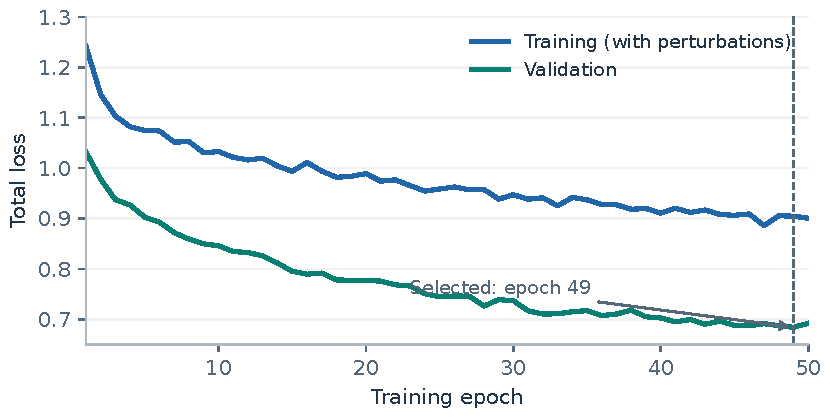
\includegraphics[width=\linewidth]{figures/training_curve.pdf}
\caption{Recorded total training and validation losses. The dashed line identifies the checkpoint selected at epoch 49. These are the weighted objectives in Equation~\eqref{eq:totalloss}, not alignment costs or certificate rates. Training includes dropout and random label remapping; validation does not.}
\label{fig:trainingcurve}
\end{figure}

Replay legality and exact optimality are evaluated outside this differentiable objective. The network learns to imitate aspects of exact solutions; the semantic checks remain explicit computations at use time. This is the reason a poor prediction may reduce candidate quality without invalidating the meaning of a successful replay or an exact certificate.
